\vspace{\presectionspace}
\section{Experiments}
\vspace{\postsectionspace}
\label{sec:experiments}
\Cref{sec:experiments_trainingdetails} describes training details, \cref{sec:experiments_mscoco,sec:experiments_drawbench} analyze results on MS-COCO and  \benchmarkname, and \cref{sec:short_further_analysis} summarizes our ablation studies and key findings. For all experiments below, the images are fair random samples from \name with no post-processing or re-ranking.


\subsection{Training details}
\vspace{-0.15cm}
\label{sec:experiments_trainingdetails}
Unless specified, we train a 2B parameter model for the $64\times64$ text-to-image synthesis, and 600M and 400M parameter models for $64\times64 \rightarrow 256\times256$ and $256\times256 \rightarrow 1024\times1024$ for super-resolution respectively. We use a batch size of 2048 and 2.5M training steps for all models. We use 256 TPU-v4 chips for our base $64\times64$ model, and 128 TPU-v4 chips for both super-resolution models. We do not find over-fitting to be an issue, and we believe further training might improve overall performance. We use Adafactor for our base $64\times64$ model, because initial comparisons with Adam suggested similar performance with much smaller memory footprint for Adafactor. For super-resolution models, we use Adam as we found Adafactor to hurt model quality in our initial ablations. For classifier-free guidance, we joint-train unconditionally via zeroing out the text embeddings with 10\% probability for all three models. We train on a combination of internal datasets, with $\approx$~460M image-text pairs, and the publicly available Laion dataset \cite{schuhmann2021laion}, with $\approx$~400M image-text pairs. There are limitations in our training data, and we refer the reader to \cref{sec:limitations} for details. See \cref{sec:impl_details_appendix} for more implementation details.

\subsection{Results on COCO}
\label{sec:experiments_mscoco}
\begin{table}[t]
\small

\parbox{.55\textwidth}{
\centering
\caption{MS-COCO $256\times256$ FID-30K. We use a guidance weight of 1.35 for our $64\times64$ model, and a guidance weight of 8.0 for our super-resolution model.}
\vspace{.2cm}
\label{tab:zero_shot_mscoco}
\begin{tabular}{lcc}
\toprule
\multirow{2}{*}{\bfseries{Model}} & \multirow{2}{*}{\bfseries{FID-30K}} & \bfseries{Zero-shot}  \\
& &  \bfseries{FID-30K} \\
\midrule
AttnGAN \citep{xu-cvpr-2018} & 35.49 & \\
DM-GAN \citep{zhu2019dm} & 32.64 & \\
DF-GAN \citep{tao2020df} & 21.42 & \\
DM-GAN + CL \citep{ye2021improving} & 20.79 & \\
XMC-GAN \citep{zhang2021cross} & 9.33 & \\
LAFITE \citep{zhou2021lafite} & 8.12 & \\
Make-A-Scene \citep{gafni2022make} & 7.55 & \\
\midrule
DALL-E \citep{ramesh-dalle} & & 17.89  \\
LAFITE \citep{zhou2021lafite} & & 26.94 \\
GLIDE \citep{nichol-glide} & & 12.24 \\
DALL-E 2 \citep{ramesh-dalle2} & & 10.39 \\
\midrule
\textbf{\name (Our Work)} & & \textbf{\ourmscocofid} \\
\bottomrule
\end{tabular}
}
\hfill
\parbox{.42\textwidth}{
\setlength{\tabcolsep}{3pt}
\centering
\caption{COCO $256\times256$ human evaluation comparing model outputs and original images. For the bottom part (no people), we filter out prompts containing one of \texttt{man}, \texttt{men}, \texttt{woman}, \texttt{women}, \texttt{person}, \texttt{people}, \texttt{child}, \texttt{adult}, \texttt{adults}, \texttt{boy}, \texttt{boys}, \texttt{girl}, \texttt{girls}, \texttt{guy}, \texttt{lady}, \texttt{ladies}, \texttt{someone}, \texttt{toddler}, \texttt{(sport) player}, \texttt{workers}, \texttt{spectators}.}
\vspace{.2cm}
\label{tab:mscoco_human_eval}
\begin{tabular}{lcc}
    \toprule
    \bfseries{Model} & \bfseries{Photorealism $\uparrow$} & \bfseries{Alignment $\uparrow$}  \\
    \midrule
    \textit{Original} \\
    \quad Original & 50.0\% & 91.9 $\pm$ 0.42 \\
    \quad \name & 39.5 $\pm$ 0.75\% & 91.4 $\pm$ 0.44 \\ 
    \midrule
    \textit{No people} \\
    \quad Original & 50.0\% & 92.2 $\pm$ 0.54 \\
    \quad \name & 43.9 $\pm$ 1.01\% & 92.1 $\pm$ 0.55 \\
    \bottomrule
    \end{tabular}
}
\end{table}




    
    





\label{sec:zero_shot_mscoco}
We evaluate \name on the COCO validation set using FID score, similar to~\citep{ramesh-dalle, nichol-glide}.
\Cref{tab:zero_shot_mscoco} displays the results. \name achieves state of the art \emph{zero-shot} FID on COCO at \ourmscocofid,  outperforming the concurrent work of DALL-E~2~\cite{ramesh-dalle2} and even models trained on COCO.
\Cref{tab:mscoco_human_eval} reports the human evaluation to test image quality and alignment on the COCO validation set. 
We report results on the original COCO validation set, as well as a filtered version in which all reference data with people have been removed. For photorealism, \name achieves 39.2\% preference rate indicating high image quality  generation.  On the set with no people, there is a boost in preference rate of \name to 43.6\%,  indicating \name's limited ability to generate photorealistic people. On caption similarity, \name's score is on-par with the original reference images, suggesting \name's ability to generate images that align well with COCO captions.

\subsection{Results on \benchmarkname}
\vspace{-0.15cm}
\label{sec:experiments_drawbench}

\begin{figure}[tb]
    \centering
    \begin{tabularx}{\linewidth}{XXXX}
        \centering
        \begin{subfigure}[t]{0.25\textwidth}
        \centering
        \hspace*{-9pt}\input{figures/pgfplots/drawit_vs_dalle2_twoway.tex}    
        \label{fig:drawit_vs_dalle2_drawbench}
        \end{subfigure} & 
        \begin{subfigure}[t]{0.25\textwidth}
        \centering
        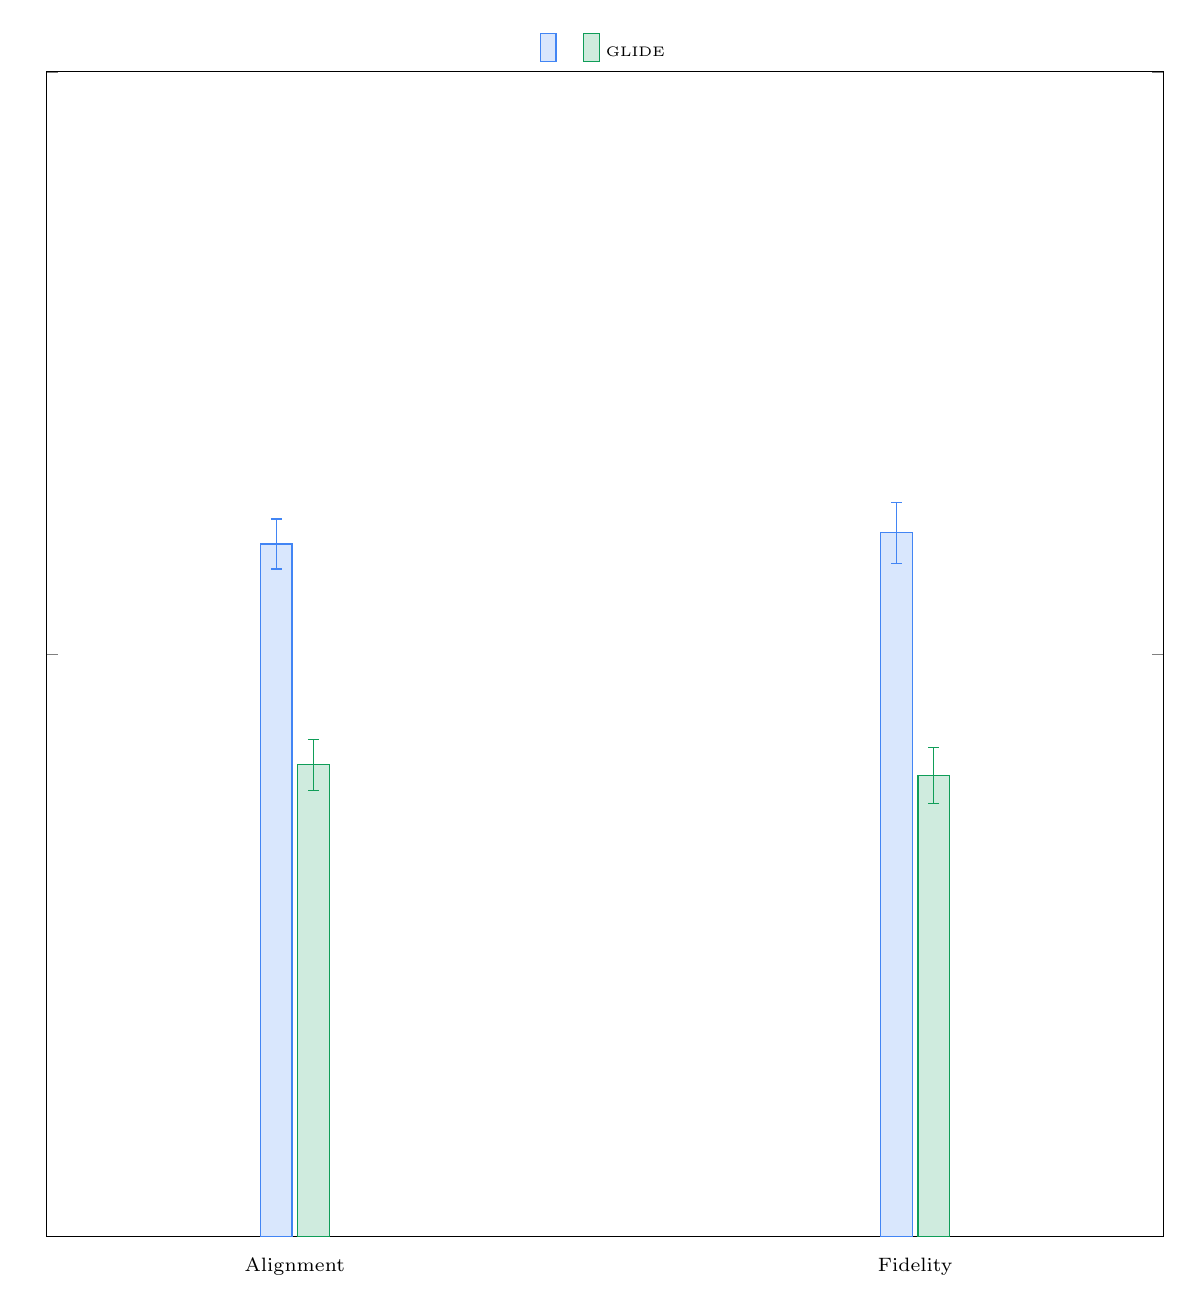
\begin{tikzpicture}

\definecolor{google_blue}{RGB}{66,133,244}
\definecolor{google_red}{RGB}{219,68,55}
\definecolor{google_yellow}{RGB}{194,144,0}
\definecolor{google_green}{RGB}{15,157,88}

\begin{axis}[
name=fidelity,
width=1.3\textwidth,
height=1.35\textwidth,
ybar,
ymin=0.0,
ymax=1.0,
xtick={1, 2},
xtick style={draw=none},
xticklabels={Alignment, Fidelity},
every tick label/.append style={font=\scriptsize},
ytick={0,0.5,1},
yticklabels={},
legend style={font=\tiny},
legend cell align=left,
legend image code/.code={
    \draw [#1] (0cm, -0.1cm) rectangle (0.2cm, 0.25cm);
},
legend style={
draw=none,
at={(0.5, 1.0)},anchor=south,
legend columns=3,
/tikz/every even column/.append style={column sep=0.2cm}
},
bar width=0.4cm,
enlarge x limits={abs=0.4},
]
\addplot+[
    fill=google_blue,
    fill opacity=0.2,
    draw=google_blue,
    error bars/error bar style={google_blue},
    error bars/.cd,
    y dir=both,
    y explicit
] coordinates {
(1.0,0.5945) +- (1.0, 0.02145839465123118)
(2.0,0.604) +- (2.0, 0.02598245656099196)
};

\addplot+[
fill=google_green,fill opacity=0.2,draw=google_green,
    error bars/error bar style={google_green},
    error bars/.cd,
    y dir=both,
    y explicit
] coordinates {
(1.0,0.405) +- (1.0, 0.021982563782935984)
(2.0,0.396) +- (2.0, 0.02406971888310527)
};


\legend{\name, GLIDE}
\end{axis}

\end{tikzpicture}


    
        \label{fig:drawit_vs_glide_drawbench}
        \end{subfigure} & 
        \begin{subfigure}[t]{0.25\textwidth}
        \centering
        \input{figures/pgfplots/drawit_vs_vqganclip_twoway}
        \label{fig:drawit_vs_vaganclip_drawbench}
        \end{subfigure} &
        \begin{subfigure}[t]{0.25\textwidth}
        \centering
        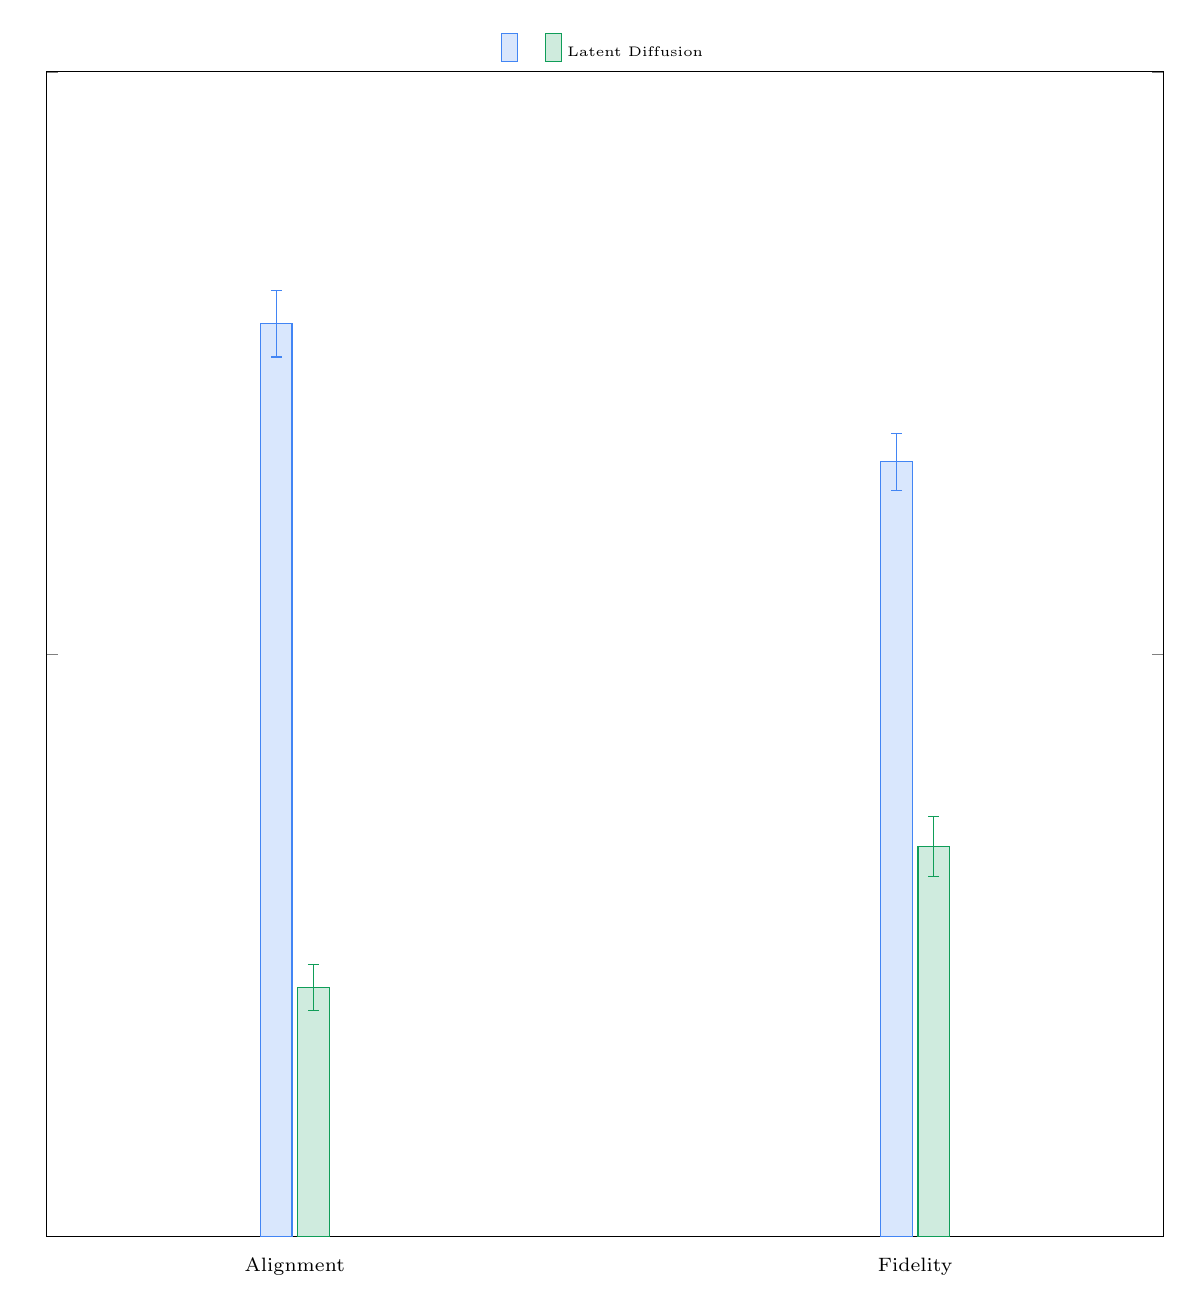
\begin{tikzpicture}

\definecolor{google_blue}{RGB}{66,133,244}
\definecolor{google_red}{RGB}{219,68,55}
\definecolor{google_yellow}{RGB}{194,144,0}
\definecolor{google_green}{RGB}{15,157,88}

\begin{axis}[
name=fidelity,
width=1.3\textwidth,
height=1.35\textwidth,
ybar,
ymin=0.0,
ymax=1.0,
xtick={1, 2},
xtick style={draw=none},
xticklabels={Alignment, Fidelity},
every tick label/.append style={font=\scriptsize},
ytick={0,0.5,1},
yticklabels={},
legend style={font=\tiny},
legend cell align=left,
legend image code/.code={
    \draw [#1] (0cm, -0.1cm) rectangle (0.2cm, 0.25cm);
},
legend style={
draw=none,
at={(0.5, 1.0)},anchor=south,
legend columns=3,
/tikz/every even column/.append style={column sep=0.2cm}
},
bar width=0.4cm,
enlarge x limits={abs=0.4},
]

\addplot+[
    fill=google_blue,
    fill opacity=0.2,
    draw=google_blue,
    error bars/error bar style={google_blue},
    error bars/.cd,
    y dir=both,
    y explicit
] coordinates {
(1.0,0.7837) +- (1.0, 0.028497994689556643)
(2.0,0.6652) +- (2.0, 0.02454522731413525)
};

\addplot+[
fill=google_green,fill opacity=0.2,draw=google_green,
    error bars/error bar style={google_green},
    error bars/.cd,
    y dir=both,
    y explicit
] coordinates {
(1.0,0.2136) +- (1.0, 0.01993785825157147)
(2.0,0.3348) +- (2.0, 0.025427213103106437)
};

\legend{\name, Latent Diffusion}
\end{axis}

\end{tikzpicture}
        \label{fig:drawit_vs_latentdiffusion_drawbench}
        \end{subfigure} \\
    \end{tabularx}
    \caption{Comparison between \name and DALL-E 2~\citep{ramesh-dalle2}, GLIDE~\citep{nichol-glide}, VQ-GAN+CLIP~\citep{crowson2022vqgan} and Latent Diffusion~\citep{rombach-cvpr-2022} on \benchmarkname: User preference rates (with 95\% confidence intervals) for image-text alignment and image fidelity.}
    \label{fig:drawbench-comparison}
    \vspace{-1em}
\end{figure}


Using \benchmarkname, we compare \name with \mbox{DALL-E 2} (the public version)~\cite{ramesh-dalle2}, \mbox{GLIDE}~\cite{nichol-glide}, \href{https://github.com/CompVis/latent-diffusion}{\color{black}{Latent Diffusion}}~\cite{rombach-cvpr-2022}, and \href{https://github.com/EleutherAI/vqgan-clip}{\color{black}{CLIP-guided VQ-GAN}}~\cite{crowson2022vqgan}. %
\cref{fig:drawbench-comparison} shows the human evaluation results for pairwise comparison of \name with each of the three models. We report the percentage of time raters prefer Model A, Model B, or are indifferent for both image fidelity and image-text alignment. We aggregate the scores across all the categories and raters. We find the human raters to exceedingly prefer \name over all others models in both image-text alignment and image fidelity. We refer the reader to \cref{sec:benchmark_comparison} for a more detailed category wise comparison and qualitative comparison. 


\subsection{Analysis of \name}
\vspace{-0.15cm}
\label{sec:short_further_analysis}
For a detailed analysis of \name see \cref{sec:experiments_analysis}. Key findings are discussed in \cref{fig:main_ablations} and below.




\textbf{Scaling text encoder size is extremely effective.} We observe that scaling the size of the text encoder leads to consistent improvement in both image-text alignment and image fidelity. \name trained with our largest text encoder, T5-XXL (4.6B parameters), yields the best results (\cref{fig:encoder_size_main_paper}).

\textbf{Scaling text encoder size is more important than U-Net size.} While scaling the size of the diffusion model U-Net improves sample quality, we found scaling the text encoder size to be significantly more impactful than the U-Net size (\cref{fig:unet_main_paper}).

\textbf{Dynamic thresholding is critical.} We show that dynamic thresholding results in samples with significantly better photorealism and alignment with text, over static or no thresholding, especially under the presence of large classifier-free guidance weights (\cref{fig:clip_vs_scaled_clip_main_paper}).

\textbf{Human raters prefer T5-XXL over CLIP on \benchmarkname.} The models trained with T5-XXL and CLIP text encoders perform similarly on the COCO validation set in terms of CLIP and FID scores. However, we find that human raters prefer T5-XXL over CLIP on \benchmarkname across all 11 categories.

\textbf{Noise conditioning augmentation is critical.} We show that training the super-resolution models with noise conditioning augmentation leads to better CLIP and FID scores. We also show that noise conditioning augmentation enables stronger text conditioning for the super-resolution model, resulting in improved CLIP and FID scores at higher guidance weights. Adding noise to the low-res image during inference along with the use of large guidance weights allows the super-resolution models to generate diverse upsampled outputs while removing artifacts from the low-res image.

\textbf{Text conditioning method is critical.} We observe that conditioning over the sequence of text embeddings with cross attention significantly outperforms simple mean or attention based pooling in both sample fidelity as well as image-text alignment.

\textbf{Efficient U-Net is critical.} Our Efficient U-Net implementation uses less memory, converges faster, and has better sample quality with faster inference.


\begin{figure}[t]
    \centering
        \begin{subfigure}[t]{0.33\textwidth}
        \centering
        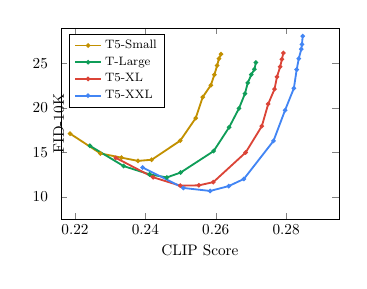
\begin{tikzpicture}[scale=0.55]
\definecolor{google_blue}{RGB}{66,133,244}
\definecolor{google_red}{RGB}{219,68,55}
\definecolor{google_yellow}{RGB}{194,144,0}
\definecolor{google_green}{RGB}{15,157,88}


\begin{axis}[
width=8cm,
height=6cm,
  xlabel=CLIP Score,
  ylabel=FID-10K,
  legend columns=1,
  legend pos=north west,
  legend cell align=left,
  y label style={at={(axis description cs:0.03,.5)}},
  legend style={font=\footnotesize},
  xmin=0.216,
  ymin=7.5,
  ymax=29,
  xmax=0.295,
  every axis plot/.append style={very thick},
  yticklabel style={xshift=-5pt}
]

\addplot +[mark=*, solid, google_yellow, mark options={scale=0.4}] coordinates {(0.2186, 17.1279)(0.2272, 14.9052)(0.2332, 14.4287)(0.2379, 14.0655)(0.2418, 14.1945)(0.2499, 16.339)(0.2543, 18.8731)(0.2563, 21.2413)(0.2586, 22.5724)(0.2596, 23.7404)(0.2604, 24.7911)(0.2609, 25.5612)(0.2615, 26.0648)};


\addplot +[mark=*, solid, google_green, mark options={scale=0.4}] coordinates {(0.2242, 15.7681)(0.2338, 13.4837)(0.2412, 12.5508)(0.2461, 12.2109)(0.25, 12.7537)(0.2594, 15.1684)(0.2638, 17.8411)(0.2666, 19.9616)(0.2683, 21.6277)(0.2691, 22.8355)(0.2701, 23.7544)(0.271, 24.3638)(0.2714, 25.1119)};


\addplot +[mark=*, solid, google_red, mark options={scale=0.4}] coordinates {(0.2316, 14.4068)(0.2422, 12.2246)(0.2499, 11.2804)(0.2552, 11.3188)(0.2593, 11.6776)(0.2685, 15.0103)(0.2731, 17.9712)(0.2749, 20.454)(0.2767, 22.132)(0.2774, 23.5054)(0.2783, 24.6424)(0.2788, 25.485)(0.2792, 26.1941)};


\addplot +[mark=*, solid, google_blue, mark options={scale=0.4}] coordinates {(0.2392, 13.33)(0.2508, 11.0229)(0.2584, 10.688)(0.2637, 11.2378)(0.268, 12.0375)(0.2764, 16.3064)(0.2797, 19.7633)(0.2822, 22.2284)(0.283, 24.3269)(0.2836, 25.5622)(0.2843, 26.6161)(0.2845, 27.1637)(0.2847, 28.0816)};



\legend{T5-Small, T-Large, T5-XL, T5-XXL}
\end{axis}
\end{tikzpicture}
        \caption{Impact of encoder size.}
        \label{fig:encoder_size_main_paper}
        \end{subfigure}%
        \begin{subfigure}[t]{0.33\textwidth}
        \centering
        \input{figures/pgfplots/model_size_pareto}
        \caption{Impact of U-Net size.}
        \label{fig:unet_main_paper}
        \end{subfigure}%
        \begin{subfigure}[t]{0.33\textwidth}
        \centering
        \input{figures/pgfplots/clip_vs_scaled_clip}
        \caption{Impact of thresholding.}
        \label{fig:clip_vs_scaled_clip_main_paper}
        \end{subfigure}
    \caption{Summary of some of the critical findings of \name with pareto curves sweeping over different guidance values. See \cref{sec:experiments_analysis} for more details.}
    \label{fig:main_ablations}
    \vspace{-1em}
\end{figure}